\documentclass{minimal}
\usepackage{graphics}
\usepackage[a4paper,hmargin=1.5cm,tmargin=2cm,bmargin=3cm]{geometry}
\begin{document}
\raggedright\noindent
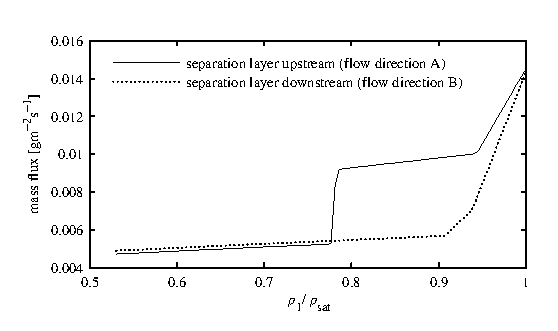
\includegraphics{figure1.eps}
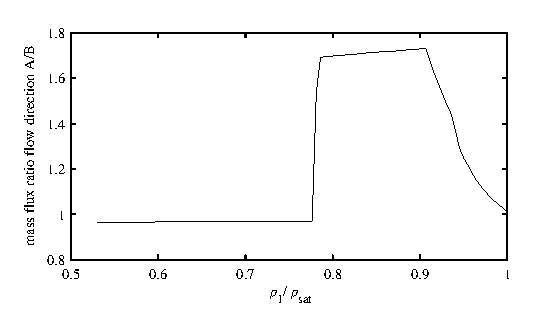
\includegraphics{figure2.eps}\\
Pressure difference 0.5~bar.
$p_\mathrm{cond}/p_\mathrm{sat}(\hbox{direction A}) = 0.78$,
$p_\mathrm{cond}/p_\mathrm{sat}(\hbox{direction B}) = 0.96$.\bigskip

\includegraphics{figure3.eps}
\includegraphics{figure4.eps}\\
Pressure difference 1~bar.
$p_\mathrm{cond}/p_\mathrm{sat}(\hbox{direction A}) = 0.74$,
$p_\mathrm{cond}/p_\mathrm{sat}(\hbox{direction B}) = 0.91$.\bigskip

\includegraphics{figure5.eps}
\includegraphics{figure6.eps}\\
Pressure difference 1.5~bar.
$p_\mathrm{cond}/p_\mathrm{sat}(\hbox{direction A}) = 0.70$,
$p_\mathrm{cond}/p_\mathrm{sat}(\hbox{direction B}) = 0.87$.\bigskip

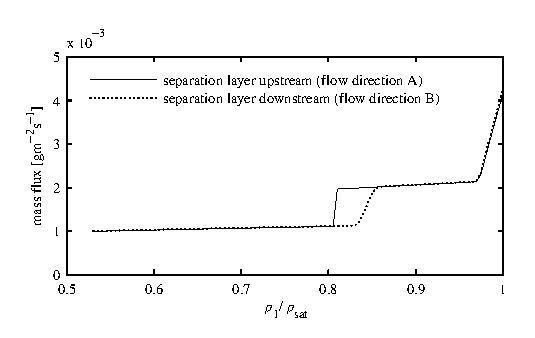
\includegraphics{figure7.eps}
\includegraphics{figure8.eps}\\
Pressure difference 0.1~bar.
$p_\mathrm{cond}/p_\mathrm{sat}(\hbox{direction A}) = 0.81$,
$p_\mathrm{cond}/p_\mathrm{sat}(\hbox{direction B}) = 0.99$.
\end{document}
